\documentclass{book}
\title{Cálculo Multivariable  - Rocket Book Compiliation}
\author{Christiaan Ketelaar \\ Organizado por : David Corzo}
\date{2020-01-06}

\usepackage[margin = 1in]{geometry}
\usepackage{graphicx}
\usepackage{fontenc}
\usepackage{pdfpages}
\usepackage[spanish]{babel}
\usepackage{amsmath}
\usepackage{amsthm}
\usepackage[utf8]{inputenc}
\usepackage{enumitem}
\usepackage{mathtools}
\usepackage{import}
\usepackage{xifthen}
\usepackage{pdfpages}
\usepackage{transparent}
\usepackage{color}
\usepackage{fancyhdr}
\usepackage{lipsum}
\usepackage{sectsty}
\usepackage{titlesec}
\usepackage{calc}
\usepackage{lmodern}
\usepackage{xpatch}
\usepackage{blindtext}
\usepackage{bookmark}
\usepackage{fancyhdr}
\usepackage{xcolor}
\usepackage{tikz}
\usepackage{blindtext}
\usepackage{hyperref}
\usepackage{listing}
\usepackage{spverbatim}
\usepackage{fancyvrb}
\usepackage{fvextra}
\usepackage{amssymb}
\usepackage{pifont}
\usepackage{longtable}
\usepackage{multirow}
\makeatletter \xpatchcmd{ \@makeschapterhead }{ \Huge \bfseries  #1\par\nobreak }{ \Huge \bfseries\centering #1\par\nobreak }{ \typeout{Patched makeschapterhead}}{\typeout{patching of @makeschapterhead failed} } \xpatchcmd{\@makechapterhead}{ \huge\bfseries \@chapapp \space \thechapter}{ \huge \bfseries \centering \@chapapp\space \thechapter }{ \typeout{Patched @makechapterhead}}{\typeout{Patching of @makechapterhead failed}}\makeatother

\fancyhead{}\fancyfoot{}{\fontfamily{mc}\selectfont\fancyfoot[L]{\thepage}\fancypagestyle{plain}{\renewcommand{\headrulewidth}{0pt}\fancyhf{}\fancyfoot[L]{\thepage}}}

\begin{document}
\maketitle
\tableofcontents

\chapter{ RB\_2020-01-07\_18\_49\_53 }
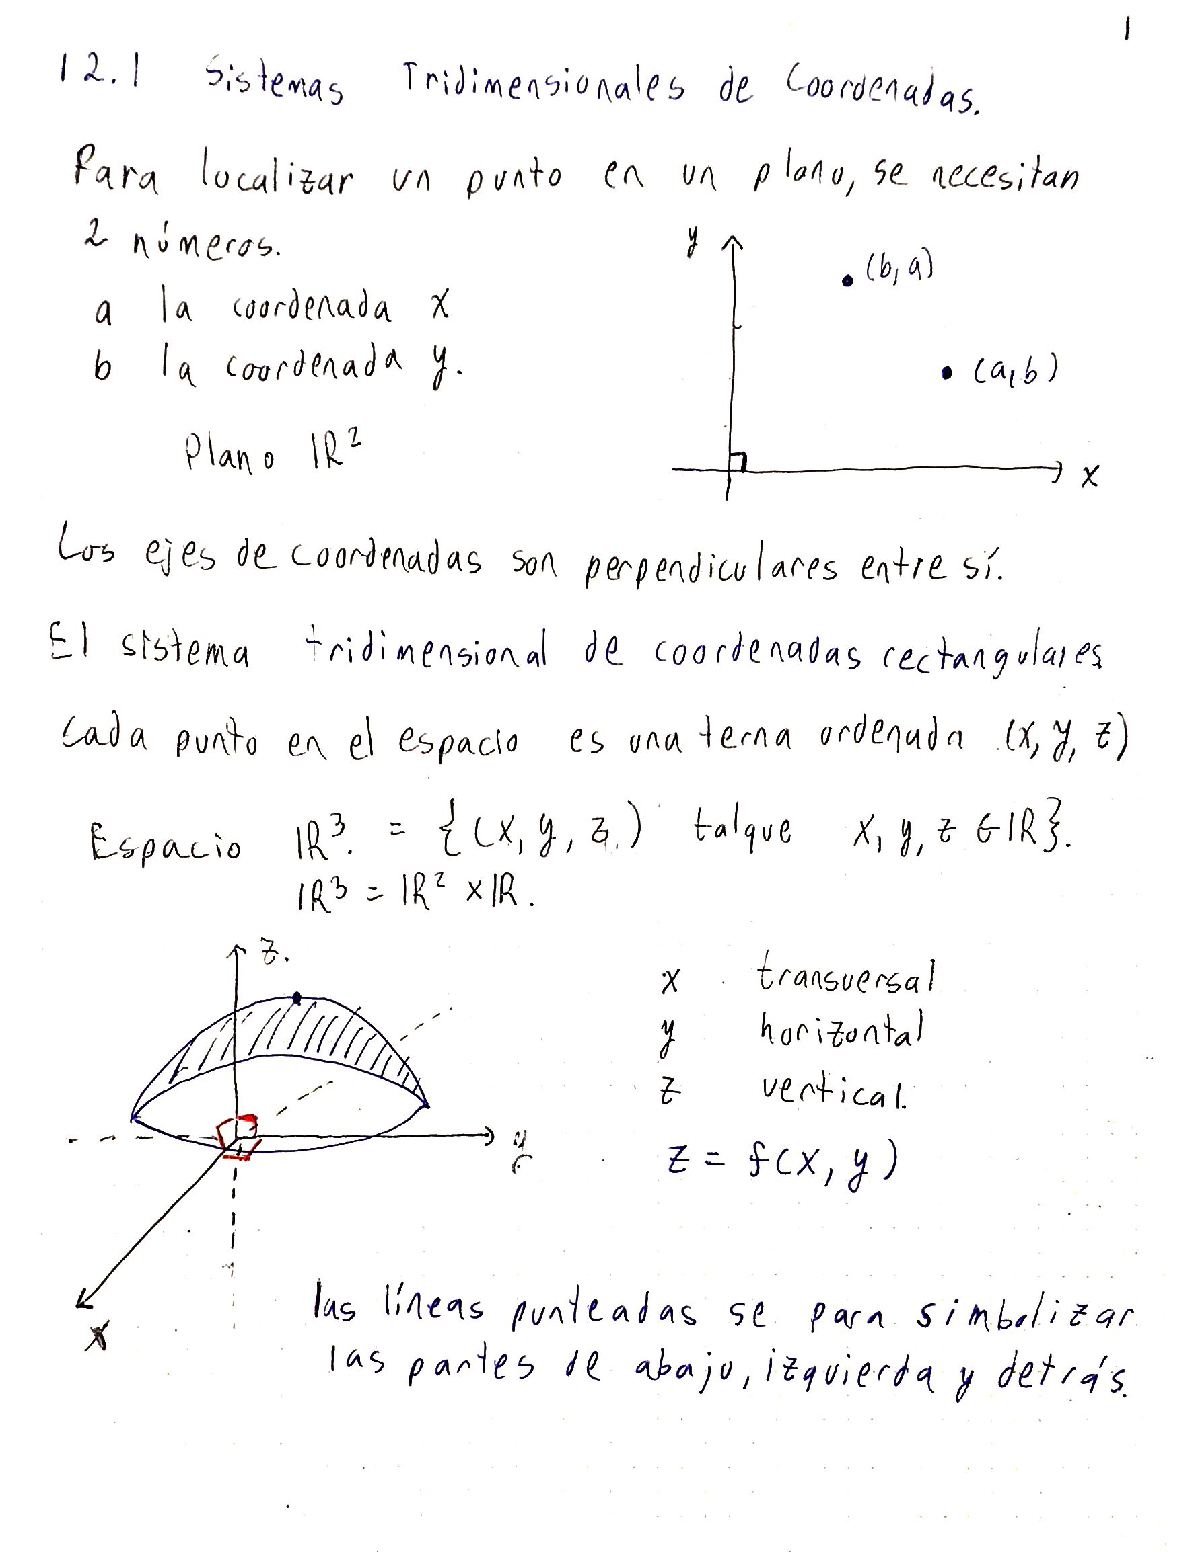
\includepdf[pages=-,pagecommand={\thispagestyle{plain}}]{RB/RB_2020-01-07_18_49_53.pdf}


%%%%%%%%%%%%%%%%%%%%%%%%%%%%%%%%%%%%%%%%%%%%%%%%%%%%%%%%%%%%%%%%%%%%%%%%%%%%%%%%%%%%%%%%%%%%%%%%

\chapter{ RB\_2020-01-09\_09\_42\_27 }
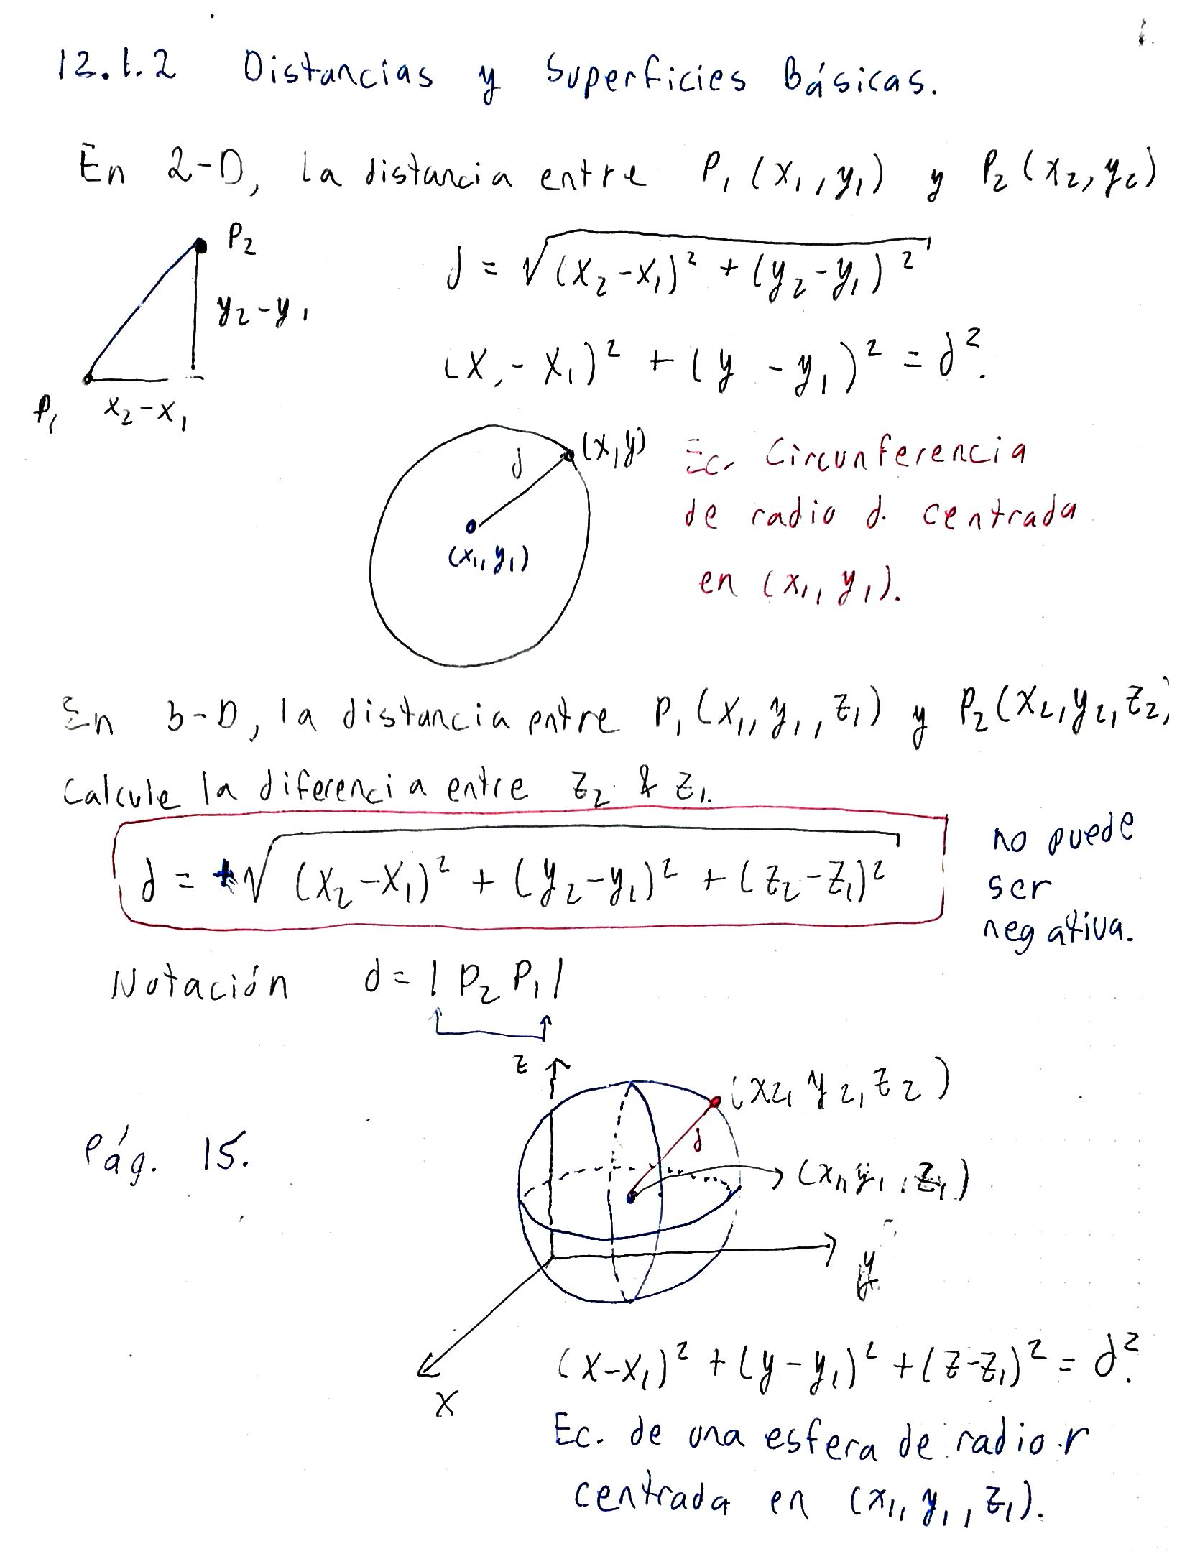
\includepdf[pages=-,pagecommand={\thispagestyle{plain}}]{RB/RB_2020-01-09_09_42_27.pdf}


%%%%%%%%%%%%%%%%%%%%%%%%%%%%%%%%%%%%%%%%%%%%%%%%%%%%%%%%%%%%%%%%%%%%%%%%%%%%%%%%%%%%%%%%%%%%%%%%

\end{document}
